\documentclass[12pt,notitlepage]{article}

\usepackage{mathtools}
\usepackage{hyperref}
\usepackage{listings}

\usepackage{newfloat}
\DeclareFloatingEnvironment[name=Example]{example}

\usepackage{subfig}

\usepackage{tikz}
\usetikzlibrary{calc}
\usetikzlibrary{positioning}

\usetikzlibrary{matrix}
\usetikzlibrary{graphs}
\usetikzlibrary{shapes}
\usetikzlibrary{arrows.meta}

\title{The SwizzleFlow algorithm}
\author{Krzysztof Drewniak}
\date{May 2019}

% Arguments are y, var, and for loop args
\tikzset{prognode/.style={shape=rectangle, minimum width=0.75cm, minimum height=0.5cm, draw=black},
  perm/.style={every edge/.append style={-Latex[]}}}

\begin{document}
\maketitle{}

SwizzleFlow is a system for synthesizing GPU kernels like those produced by Swizzle Inventor[SwInv cite].
It improves on previous work by having significantly higher performance and being much more scaleable. \textbf{[[TODO, make things more parallel to actually prove that]]}.
SwizzleFlow achieves these results through a novel method for pruning an enumerative search called \emph{abstract dynamic programming}.
Using this method, we can reject most infeasible intermediate solutions, even though the state space for the search is large, by referring to a precomputed cache of paths through an abstract program domain.

\section{Program states}
Consider the following program,
\begin{example}
\begin{verbatim}
#define T 4
parallel for (t = 0; t < T; i++) {
    int x = load(input + t);
    x = shuffle(x, (3 * t) % T);
    x = shuffle(x, (t + 1) % T);
    store(input + t, x);
}
\end{verbatim}
  \caption{Simple example program}
  \label{ex:intro}
\end{example}

where $\operatorname{shuffle}(x, i)$ broadcasts the value $x$ to all threads and reads a broadcast value from thread $i$.

This simple program will serve to illustrate the terminology we use for more complex GPU kernels, which often take on a variation of this form.

The first observation we can make is that, if we consider each thread separately, the body of the loop can be easily converted to single static assignment (SSA) form.
We can then consider how data flows between the threads (using $x_i$ to represent the inputs), as shown in Figure~\ref{fig:concrete_ex_intro-a}..



\begin{figure}
  \centering
  \subfloat[Data flow]{%
    \label{fig:concrete_ex_intro-a}%
    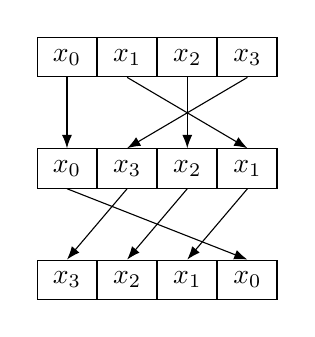
\begin{tikzpicture}
    \matrix (x) [ampersand replacement=\&, matrix of math nodes, nodes={prognode}, row sep=0.9cm] {
      x_0 \& x_1 \& x_2 \& x_3\\
      x_0 \& x_3 \& x_2 \& x_1\\
      x_3 \& x_2 \& x_1 \& x_0\\
    };
    \draw[perm]
    (x-1-1.south) edge (x-2-1.north)
    (x-1-2.south) edge (x-2-4.north)
    (x-1-3.south) edge (x-2-3.north)
    (x-1-4.south) edge (x-2-2.north);

    \draw[perm]
    (x-2-1.south) edge (x-3-4.north)
    (x-2-2.south) edge (x-3-1.north)
    (x-2-3.south) edge (x-3-2.north)
    (x-2-4.south) edge (x-3-3.north);
  \end{tikzpicture}}%
\qquad
\subfloat[Program graph]{%
  \label{fig:concrete_ex_intro-b}%
  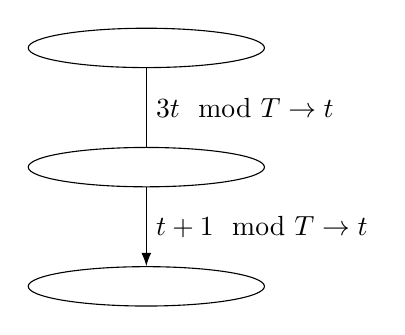
\begin{tikzpicture}
    \draw[{-Latex[]}, item/.style={draw, ellipse, minimum height=0.5cm, minimum width=3cm}]
    node[item] (a) {}
    node[item, below = 1cm of a.south] (b) {}
    node[item, below = 1cm of b.south] (c) {}
    (a) -- (b) node[midway,right] {$3t \mod T \to t$}
    (b) -- (c) node[midway, right] {$t + 1 \mod T \to t$};
  \end{tikzpicture}}
  \caption{Illustrations for Example~\ref{ex:intro}} %
  \label{fig:concrete_ex_intro}
\end{figure}
\end{document}
